\label{chapter:applications}

In this chapter we discuss applications of our improvements to the binary XPFC
model.  To begin we'll discuss an effective equation of motion in the limit
that density change on solidification is small, after which we'll examine the
to process of multi-step nucleation of nanoparticles from solution. To conclude
we'll discuss areas of future application.

%%%%%%%%%%%%%%%%%%%%%%%
\subsection{Dynamics} %
%%%%%%%%%%%%%%%%%%%%%%%

To examine applications of our improvements to the XPFC model we begin by
considering equations of motion. Following \cite{GREENWOOD11_BINARY}, we use
conservative dynamics for both $n(x, t)$ and $c(x, t)$.
%
\begin{gather}
    \f{\partial n(x, t)}{\partial t} = 
        M_n \nabla^2\l(\f{\d \beta \Delta\F / \rho_0}{\d n(x, t)}\r) 
        + \xi_n(x, t), \\ 
    \f{\partial c(x, t)}{\partial t} = 
        M_c \nabla^2\l(\f{\d \beta \Delta \F / \rho_0}{\d c(x, t)}\r)
        + \xi_c(x, t).
\end{gather}
%
These equations of motion are largely phenomenological as, strictly speaking,
there is no reason that the local concentration should be conserved.  This
conservation can be justified in the limit that the total density does not
deviate far from the reference. When this is the case we have $c \equiv \B /
\rho \approx \B / \rho_0$ which \textit{is} conserved.

%%%%%%%%%%%%%%%%%%%%%%%%%%%%%%%%%%%%%%%%%%%%%%%%%%%%%%%%%%%%%
\section{Multistep Nucleation of Nanoparticles in Solution} %
%%%%%%%%%%%%%%%%%%%%%%%%%%%%%%%%%%%%%%%%%%%%%%%%%%%%%%%%%%%%%

Recent experimental work has shown that precipitation of nanoparticles solution
can follow a pathway vary different from that assumed by Classical Nucleation
Theory (CNT).  In gold and silver nanoparticles\cite{LOH17} as well as calcium
carbonate (CaCO${}_3$)\cite{WALLACE13} systems precipitation occurs first via
spinodal decomposition of the aqueous solution followed by nucleation inside
the resulting solute-rich liquid droplets. CNT assumes that, for binary
systems, assumes that changes in order and composition occur simultaneously.
While there is some dispute about whether or not to call this process a
non-classical nucleation pathway \cite{DAVEY13, GEBAUER11}, the observed pathway
to precipitation raises several questions regardless of semantics about its
classification. Under what conditions does this pathway occur? How does the 
pathway effect the polydispersity of the final nanoparticle? We present here
initial finding using the improved binary XPFC formalism.

These experimental findings are among many works that point to a deficiency in
CNT. Common among these works is the presence of a multi-step nucleation
process. While some theoretical description exist for these multi-step
processes, they typically posit highly simplified pathways to nucleation for
simplicity of analysis that may be far from the actual kinetics experienced by
the system.  For instance in the study of condensation of a pure material,
Lutsko \textit{et al.} \cite{LUTSKO15} restricted the nucleus to a spherical
droplet with radius $R$ and density $\rho$. Thus restricted, they find that the
most likely path to nucleation follows a three-stage pathway.  These theories
can justify a multi-step nucleation pathway but do little more to advance our
knowledge of the \textit{actual} pathway to nucleation.

It is important, then, to have robust models that contain all of the essential
physics of these systems to gain a deeper insight into the phenomena. The works
of Loh \cite{LOH17} are a special case of diffusion limited precipitation because
their system was a 30nm thick aqueous solution. The effective diffusion
constant in this thin water film is 9 orders of magnitude smaller than in the
bulk and as such the system is diffusion limited. To model this process we must
be able to  model changes in composition, structure and density. A negative
enthalpy of mixing is clearly playing in important role so our improved XPFC
model is a good fit.

To construct an appropriate free energy functional for this system we consider
the structure of its equilibrium phase diagram. Precipitation is indicative of
a simple liquid-solid coexistance curve beneath which we assume there also a 
submerged metastable liquid spinodal \cite{DAVEY13}. Producing a system with
these characteristics is similar to that of a monotectic with the exception
that the spinodal temperature, $T_c$, must now be sufficiently low to hide
below the coexistance curve. We will also also use a Gaussian window function
$\zeta(c)$ as the in the monotectic case though this time centring the Gaussian
about $c = 1$ in keeping with interpreting the concentration as a solute
concentration.  An example, including depiction of the metastable spinodal, can
be seen in figure \ref{fig:precip_phase_dia}.

\begin{figure}
    \centering	
    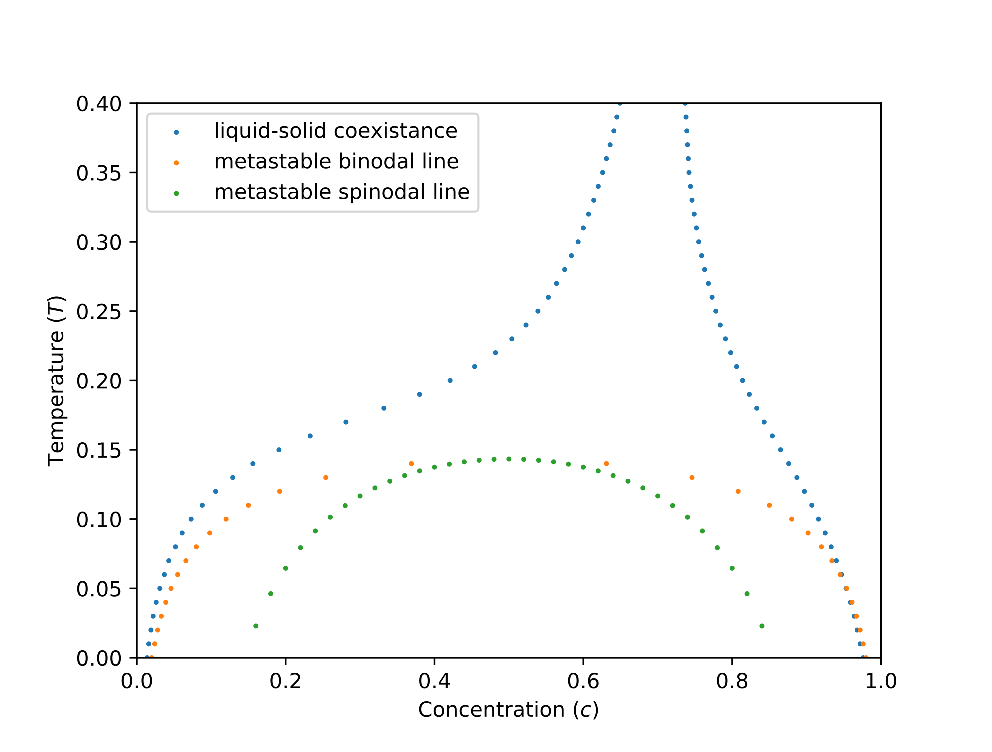
\includegraphics[scale=0.6]{solution.eps}
    \caption[Coexistance Phase Diagram with Metastable Spinodal]{
        \label{fig:precip_phase_dia} Phase Diagram of Solution \color{ForestGreen} fill
        me in please!!
    }
\end{figure}

We would expect that, starting from a uniform initial condition, if we quench
the system through the coexistance region and past the liquid spinodal we might
see a nucleation pathway similar to that observed experimentally. Results of a
numerical simulation \footnote{See appendix \ref{appendix:algorithm} for a
detailed description of the integration algorithm} can be seen in figure
\ref{fig:precipitation}. We see that, much as in experimental observation,
nanoparticle nucleation is preceded by spinodal decomposition.

\begin{figure}
    \centering
    \begin{subfigure}[b]{0.3\textwidth}
        
\includegraphics[width=\textwidth]{initial}
        \label{fig:initial}
        \caption{}
    \end{subfigure}
    ~
    \begin{subfigure}[b]{0.3\textwidth}
        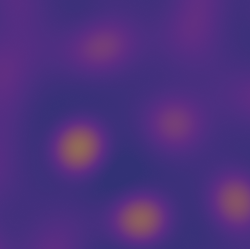
\includegraphics[width=\textwidth]{early_spinodal}
        \label{fig:early_spinodal}
        \caption{}
    \end{subfigure}
    ~
    \begin{subfigure}[b]{0.3\textwidth}
        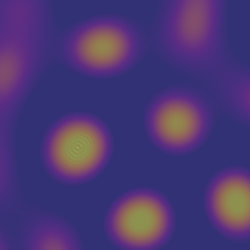
\includegraphics[width=\textwidth]{devel_spinodal.png}
        \label{fig:devel_spinodal}
        \caption{}
    \end{subfigure}

    \vspace{0.25cm}
    \begin{subfigure}[b]{0.3\textwidth}
        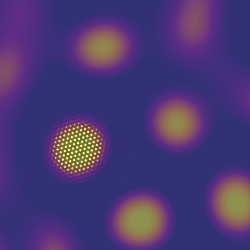
\includegraphics[width=\textwidth]{nucleation}
        \label{fig:nucleation}
        \caption{}
    \end{subfigure}
    ~
    \begin{subfigure}[b]{0.3\textwidth}
        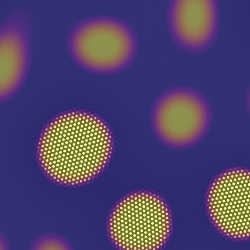
\includegraphics[width=\textwidth]{nucleation_and_sacrificial_growth}
        \label{fig:nucleation_and_growth}
        \caption{} 
    \end{subfigure}
    ~
    \begin{subfigure}[b]{0.3\textwidth}
        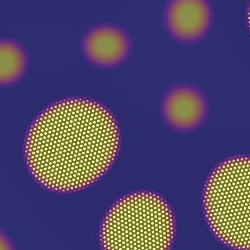
\includegraphics[width=\textwidth]{sacrificalgrowth}
        \label{fig:sacrifical_growth}
        \caption{}
    \end{subfigure}
    
    \vspace{0.25cm}
    \begin{subfigure}[b]{0.3\textwidth}
        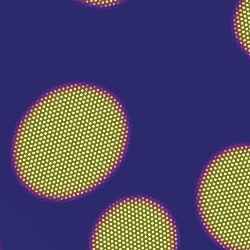
\includegraphics[width=\textwidth]{crystalgrowth}
        \label{fig:crystalgrowth}
        \caption{}
    \end{subfigure}
    ~
    \begin{subfigure}[b]{0.3\textwidth}
        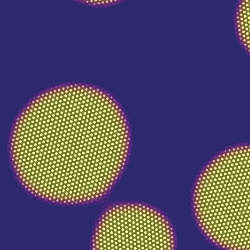
\includegraphics[width=\textwidth]{crystalgrowth2}
        \label{fig:crystalgrowth2}
        \caption{}
    \end{subfigure}
    ~ 
    \begin{subfigure}[b]{0.3\textwidth}
        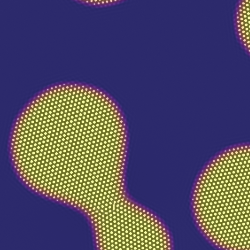
\includegraphics[width=\textwidth]{crystalgrowth3}
        \label{fig:crystalgrowth3}
        \caption{}
    \end{subfigure}
    \caption[Stages of precipitation of nanoparticles from solution]{
        \label{fig:precipitation}
        Various stages of precipitation of nanoparticles from solution. All
        thermodynamic parameters are shared with figure
        \ref{fig:precip_phase_dia}. The initial condition is a uniform solution
        quenched abruptly to $T$ = 0.07. The initial condition has
        concentration $c = 0.3$ and relative density $n = 0.05$. Mobilities
        $M_n$ and $M_c$ are set to 1 and $W_c$ is set to 3.0. Numerical
        parameters are grid spacing $\Delta x = 0.125$ on a 1024 by 1024
        lattice with time step size $\Delta t = 0.0025$. Sub-figures (a) - (c)
        show spinodal decomposition of the liquid into solute right and solute
        poor regions. Sub-figures (d) - (f) show nucleation of the solid and
        solid growth at the expense of liquid regions.  The remaining
        sub-figures show only nanoparticle growth and coarsening.
    }
\end{figure}

Our model finds some addition complexity in the nucleation process as well.
Once crystalline nuclei start to form, they growth is accelerated at the
expense of the solute-rich liquid droplets in solution. In a system of coarsen
droplets with only a single phase, larger droplets grow at the expense of
smaller droplets to reduce the total surface tension in the system. This
process is called Oswald ripening. In the nanoparticle system even smaller
crystalline particles can grow at the expense of larger liquid droplets due to
their difference in chemical potential.

\begin{figure}
    \centering
    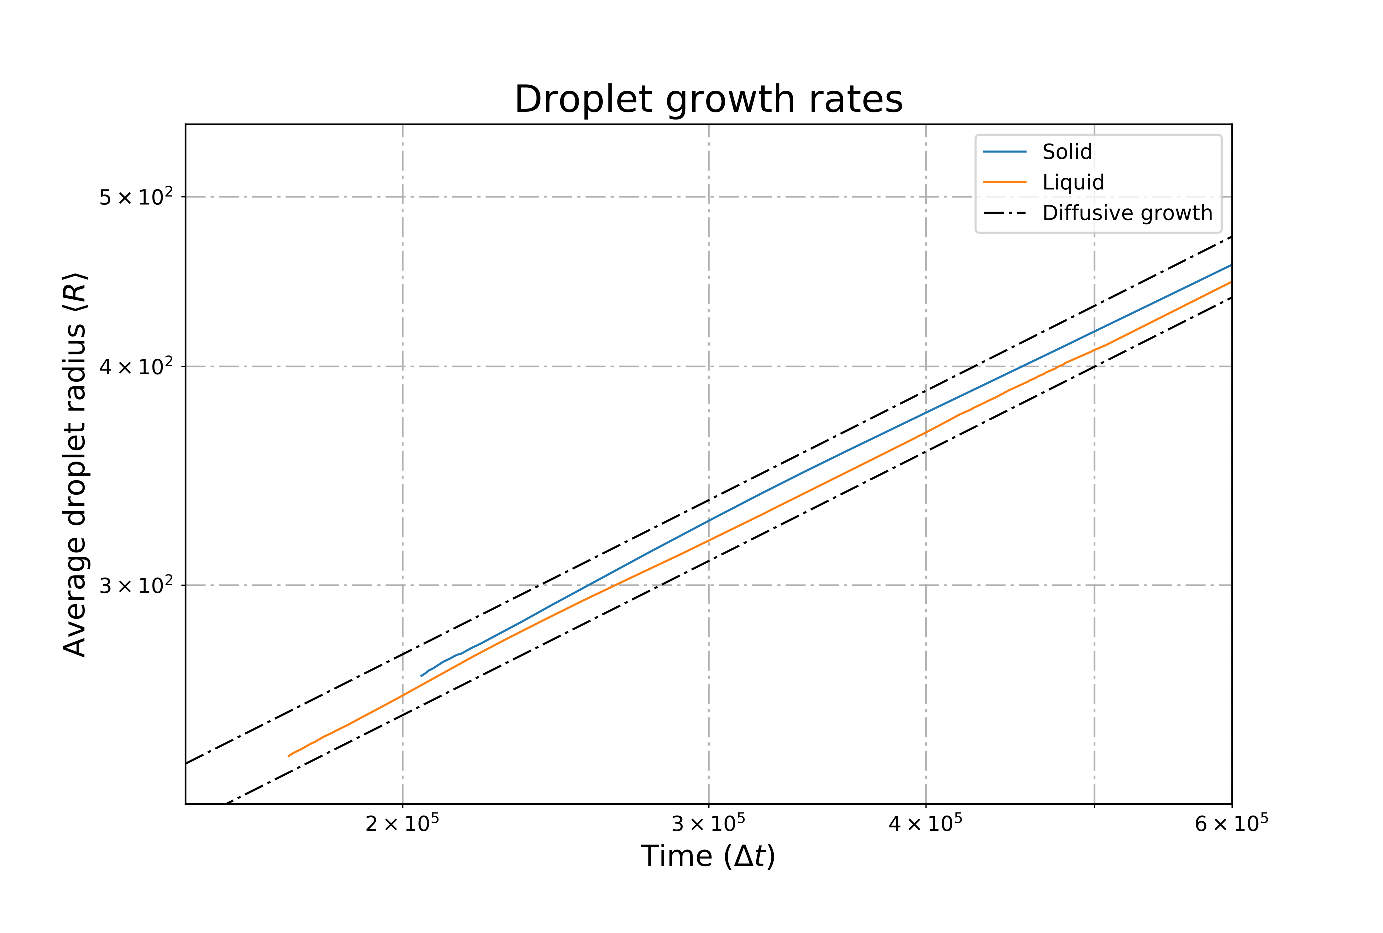
\includegraphics[width=\textwidth]{scaling}
    \caption{
        \label{fig:scaling}
        Droplet growth exponents
    }
\end{figure}

We can examine this growth phenomena more systematically by measuring the
ensemble average droplet radius $\langle R(t) \rangle$ over time. We achieve
this by running 120 simulations with the same parameters as the quench
described in figure \ref{fig:precipitation} and computing the radius of all
droplets and their phase (liquid or solid) throughout the simulation. Strictly
diffusive growth scales like $\mean{R(t)} \sim t^{1/2}$ and so in plotting the
mean radius versus time on a log-log plot as in figure \ref{fig:scaling} we see
how the growth of solid and liquid droplets compare to diffusive growth. Early
solid droplets grow at a weakly hyper-diffusive rate due to the presence of
the sacrificial liquid droplets and slow to sub-diffusive as they begin to
coarsen.

\begin{figure}
    \centering
    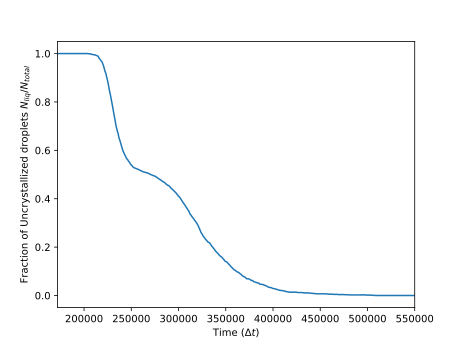
\includegraphics[width=0.7\textwidth]{incubation}
    \caption[Fraction of uncrystallized droplets in time]{
        \label{fig:incubation}
        Fraction of uncrystallized droplets in time
    }
\end{figure}

A more pronounced view of this phenomena can be seen by examining the fraction
of uncrystallized droplets in the system with respect to time as in figure
\ref{fig:incubation}. Neither classical nor proposed non-classical nucleation
theories explain the pronounced reduction in nucleation rate seen once the
fraction of solid droplets reachs approximately one half. Instead of developing
via nucleation in the remaining droplets we see liquid droplet anhilation
beginning to become an important driving factor in increasing the solid
fraction. As liquid droplets shrink the nucleation rate inside the droplet is
suppressed by solute and density segregation to solid droplets. In classical
nucleation theory we would expect an exponential decay and even in proposed
two-step mechanisms do not account for these solid-liquid droplet effects\cite{MYERSON04, MYERSON09}.


